\documentclass[conference]{IEEEtran}
\IEEEoverridecommandlockouts

\usepackage{cite}
\usepackage{amsmath,amssymb}
\usepackage{graphicx}
\usepackage{booktabs}
\usepackage{array}
\usepackage{url}
\usepackage{xcolor}

\graphicspath{{figures/ieee/}}
\newcommand{\pct}{\,\%}

\begin{document}

\title{An Agentic Content Moderation System with a Fail-Closed, Age-Aware Recommendation Gate}

% TODO before submission: replace every field in this author block.
\author{\IEEEauthorblockN{First Author}
\IEEEauthorblockA{\textit{Department} \\
\textit{Institution}\\
City, Country \\
email@example.com}
\and
\IEEEauthorblockN{Second Author}
\IEEEauthorblockA{\textit{Department} \\
\textit{Institution}\\
City, Country \\
email@example.com}}

\maketitle

\begin{abstract}
Automated content moderation has long relied on supervised classifiers that need large labelled datasets and return one score for one kind of harm. We describe a platform that moves from that data-heavy design to an agentic one: six cooperating agents built on a language model call a toxicity classifier, policy rules and a memory of past cases as tools, and hand unsettled items to a human moderator. Every submission is moderated, rated and checked before it can reach any viewer. On top of this pipeline we add an age-aware recommender. The pipeline's outputs are combined into an audience rating (all ages, teen, adult or blocked) by rules that can only raise the rating, so a missing or malformed signal never widens an item's audience. A deterministic, fail-closed gate of ten ordered checks then runs before and after every learned ranking component, so no learned signal can admit an item. We evaluate on seeded synthetic data: 800 items, 80 viewer profiles and 200 resolved moderation cases. In 64,000 profile--item decisions and 1,040 generated feeds, no item above the viewer's age tier was served, while 94.3\pct{} of clean child items and 95.8\pct{} of clean teen items still reached their audience. With the gate removed, 96.9\pct{} of child feeds and 66.4\pct{} of teen feeds contained a forbidden item. A gate decision took about 23\,$\mu$s and a full feed request 19\,ms (median) on a laptop CPU. The learned ranking added little over an interest-only sort. Three adversarial reviews found twelve leaks, all fixed, and a run through the real pipeline exposed two defects that every synthetic test had passed. The language model itself is not part of any measured result, and the gate enforces ratings without validating them.
\end{abstract}

\begin{IEEEkeywords}
content moderation, agentic AI, multi-agent systems, age-appropriate recommendation, child safety, human-in-the-loop, fail-closed design, Thompson sampling
\end{IEEEkeywords}

\section{Introduction}

Online platforms run two automated systems over the same content. A moderation system decides whether an item may stay, and a recommender decides which of the remaining items each user sees. For most of the past decade the first of these has been a supervised classifier. Such a model is trained on a large labelled corpus for one kind of harm, returns one score, and must be relabelled and retrained when language or policy changes \cite{gorwa2020algorithmic,kotarcic2022human}. A toxicity model does not recognise spam, a sensitive topic or a policy that was written last month, and it gives a moderator no reason for its score.

Agentic architectures offer a different arrangement. A language-model agent reasons over a submission, calls tools, and explains its verdict \cite{yao2023react,piot2025watched}. The classifier does not disappear; it becomes one tool among several, alongside policy rules, retrieval of similar past cases and a human reviewer. The platform we build on made this shift. Its pipeline has six agents and a human-in-the-loop checkpoint, and every submission passes through it before publication.

Neither design answers a third question: who may see an item? Content that is acceptable for an adult can be unsuitable for a twelve-year-old, and minors commonly share feeds with adults. Ungruh \cite{ungruh2025recommender} argues that recommender research is built around adult users and overlooks children, and regulation now expects platforms to account for minors in how content is selected \cite{coppa1998,ico2020aadc,eu2022dsa}. One response is to teach the ranking model about age. The difficulty is verification: a learned model that usually demotes unsuitable items gives no statement that can be tested exhaustively, and its behaviour shifts as it learns from engagement. Agentic pipelines add a second difficulty. Their output is often incomplete: a field is missing, a category is free-form text, an agent did not run. A design that reads a missing signal as ``nothing found'' fails open.

This paper keeps the age decision outside every learned component. The agentic pipeline produces signals; a deterministic rule layer turns them into an audience rating and a gate decision; learned ranking operates only on what the gate has passed. The contributions are:

\begin{itemize}
\item an end-to-end architecture in which content is moderated by agents, rated, and gated before it reaches a viewer, and in which no learned component can admit an item to a minor's feed;
\item a method for deriving an audience rating from an agentic pipeline's existing outputs, with a fail-closed property tested by deleting and corrupting each input field;
\item an evaluation approach for such a gate (an exhaustive sweep, randomised invariants against an independent oracle, and adversarial review) with the review's findings reported;
\item measured results on synthetic data, including the negative result that learned ranking added little over an interest-only sort while the deterministic layer did all of the safety work.
\end{itemize}

Every technique used is established; the contribution is the arrangement and its evaluation. The system is a prototype and all evaluation data is synthetic. We do not measure whether the agentic pipeline classifies content more accurately than a supervised model, and we state in Section~\ref{sec:limits} what else the evidence does not support.

\section{Related Work}

\textbf{From classifiers to agents.} Gorwa \emph{et al.} \cite{gorwa2020algorithmic} and Gillespie \cite{gillespie2018custodians} describe how platforms moved moderation from human review toward automated classification and the problems that followed. Transformer classifiers such as BERT \cite{devlin2019bert} and the Detoxify models \cite{hanu2020detoxify} are standard for toxicity scoring. Recent systems wrap such classifiers in language-model agents that call tools and explain their verdicts in the ReAct pattern \cite{yao2023react}. WATCHED \cite{piot2025watched}, a preprint, is a moderator-facing agent that combines a BERT classifier, retrieval of labelled examples, a slang lookup and platform guidelines. Our host pipeline follows the same pattern, and our precedent retrieval is close to WATCHED's retrieval of similar examples.

\textbf{Human-in-the-loop moderation.} Kotarcic \emph{et al.} \cite{kotarcic2022human} document a hate-speech pipeline from annotation to a twelve-month post-deployment evaluation and find that continuous human maintenance is needed to stay robust. We take two things from this: moderator decisions update the system, and evaluation before deployment is not enough.

\textbf{Recommendation for children.} Ungruh \cite{ungruh2025recommender} sets out a research plan for child-aware recommenders, arguing that current algorithms and their evaluation target adults. That work identifies the gap and proposes audits. We build and test one mechanism for it: a rule layer that bounds what a recommender may serve to a minor. What children would find valuable remains open.

\textbf{Beyond-accuracy evaluation.} Wu \emph{et al.} \cite{wu2023fairness} survey fairness evaluation for recommenders; we cite it as background for evaluating a recommender on more than relevance, and our system does not measure fairness. The drift guard is motivated by work on filter bubbles \cite{pariser2011filter} and pathways toward more extreme content \cite{ribeiro2020auditing}; the diversity guard is a simple form of diversity-aware re-ranking \cite{carbonell1998use}.

\textbf{Techniques used.} Relevance is TF-IDF with cosine similarity \cite{salton1988term}, measured with NDCG \cite{jarvelin2002cumulated}. Exploration is Thompson sampling \cite{thompson1933likelihood,chapelle2011empirical}, as in bandit approaches to news recommendation \cite{li2010contextual}. The uncertainty margin treats disagreement among agents as uncertainty, in the spirit of ensembles \cite{lakshminarayanan2017simple}, and withholds an item when uncertain, as in selective classification \cite{geifman2017selective}. Precedent retrieval is case-based reasoning \cite{aamodt1994case}.

\section{System Architecture}

Fig.~\ref{fig:arch} shows the data flow. The design has two principles. First, \emph{moderate before serving}: an item enters the recommender only after the agentic pipeline has produced a status and a rating, and only items with an approved status can be served. Second, \emph{the gate brackets the learner}: the two gate stages are the same deterministic code, and nothing between them can add an item. Learned components only reorder or drop gate survivors.

\begin{figure*}[t]
\centering
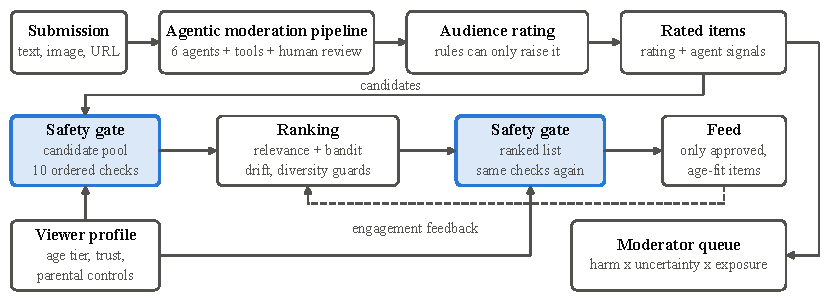
\includegraphics[width=\textwidth]{fig_architecture}
\caption{Data flow. Every submission is moderated and rated before it becomes a candidate. The same safety gate runs on the candidate pool and on the ranked list, so the ranker between them can only reorder or drop. Viewer engagement (dashed) reaches the ranker but never the gate.}
\label{fig:arch}
\end{figure*}

\subsection{From a Classifier to an Agentic Pipeline}

The host platform is a LangGraph state machine with ten nodes. Six agents carry the decision: content analysis, toxicity detection, policy checking, a ReAct-style synthesis of the earlier verdicts, user reputation scoring and action enforcement. The agents use a Google Gemini language model. A BERT-based toxicity classifier (\texttt{unitary/toxic-bert}), keyword detectors, image heuristics and a ChromaDB vector memory of past decisions are tools the agents call, not the decision-maker. A human-in-the-loop node pauses items the agents cannot settle, and an appeals path lets users contest a removal. The backend exposes 58 HTTP endpoints and six user roles.

Each agent appends a verdict and a confidence to a shared state. Final statuses include approved, flagged, under review, pending human review, warned and removed. Policy violations come from a fixed set of seven (hate speech, harassment, violence, spam, sexual content, misinformation, self-harm), while the content category is free-form text from the language model. This pipeline predates the present work; our contribution starts at its output.

\subsection{Audience Rating}

Ratings are ordered $\text{all ages} < \text{teen} < \text{adult} < \text{blocked}$. Derivation starts at all ages and applies the rules in Table~\ref{tab:rating}. Each rule can only raise the rating, so the result is the strictest rating any rule demands.

\begin{table}[t]
\caption{Rating rules. Each rule can only raise the rating.}
\label{tab:rating}
\centering
\footnotesize
\begin{tabular}{@{}p{0.63\columnwidth}p{0.29\columnwidth}@{}}
\toprule
Signal & Effect \\
\midrule
Removed, or author sanctioned & blocked \\
Status not exactly ``approved'' & at least adult \\
High-risk category, no human approval & blocked \\
High-risk category, human-approved & at least adult \\
Toxicity $\ge 0.75$ / $\ge 0.35$ / $\ge 0.10$ & blocked / adult / teen \\
Toxicity missing or outside $[0,1]$ & at least adult \\
Violation other than spam or copyright & at least adult \\
Spam or copyright violation & at least teen \\
Any policy flag; severity medium or unknown & at least adult \\
Sensitive, explicit, hate or harassment flag not exactly false & at least adult \\
Media risk above ``low'' & at least adult \\
A judging agent did not allow, no human approval & at least adult \\
Topic not on the teen list, or no topic & at least adult \\
Topic on the teen list, not the child list & at least teen \\
\bottomrule
\end{tabular}
\end{table}

\emph{Fail-closed property.} For every input field, a missing, null, wrongly typed or unrecognised value yields a rating at least as strict as any valid value. We test this by deleting and corrupting each field in turn.

\emph{Agent agreement.} Two further signals are kept for the gate. Disagreement is $d = 1 - g/n$, where $n$ is the number of judging agents and $g$ the size of the largest verdict group. Confidence $c$ is the lowest confidence a judging agent reported. A final human approval sets $d = 0$.

\emph{Human override.} A moderator's decision outranks a later machine rating. Approval alone rates an item adult at most. An item a moderator has both approved and tagged by hand is rated from those tags, with the machine signals still able to raise the rating.

\subsection{The Safety Gate}

A viewer profile holds an age tier ($\text{child} < \text{teen} < \text{adult}$), a trust level for that tier, optional parental controls and the viewer's interests. Only the age group is stored, not a date of birth. For a viewer and an item, the checks in Table~\ref{tab:gate} run in order and the first failure rejects the item with a reason code.

\begin{table}[t]
\caption{Gate checks, in order.}
\label{tab:gate}
\centering
\footnotesize
\begin{tabular}{@{}rp{0.56\columnwidth}p{0.27\columnwidth}@{}}
\toprule
\# & Reject when & Applies to \\
\midrule
1 & Rated blocked, or removed or banned status & everyone \\
2 & Status not approved or warned & everyone \\
3 & No rating & minors; self-declared adults \\
4 & Parental blocked topic or rating cap & profiles with controls \\
5 & High-risk category label & child, teen \\
6 & Rating rank above tier rank & everyone \\
7 & Topic off the tier allow-list, disallowed violation, or toxicity over the tier limit & child, teen \\
8 & Sensitive teen topic without parental allowance & child, teen \\
9 & Borderline item & child; teen under strict controls \\
10 & Status not exactly approved, signals missing, or uncertainty too high & child, teen, self-declared adult \\
\bottomrule
\end{tabular}
\end{table}

Check 10 applies an uncertainty margin. An item is rejected when
\begin{equation}
d \ge T \quad \text{or} \quad c < 1 - T, \qquad T = 0.45 \, \tau \, \sigma ,
\label{eq:margin}
\end{equation}
where trust $\tau$ is 1.0 for a verified age, 0.85 for a parent-linked account and 0.7 for a self-declared age, and strictness $\sigma$ is 1.0, 0.8 or 0.6 for low, medium or strict parental controls. The threshold therefore ranges from $T = 0.45$ down to $T = 0.189$: lower trust in the declared age narrows what is served, and so does a stricter parental setting.

Four properties follow from the design. \emph{Independence}: the gate reads tier, trust and parental controls only; interests, learned weights, feed history and bandit state are not inputs. \emph{Defence in depth}: checks 5 and 7 repeat conditions the rating already encodes, so a wrong or stale rating alone cannot expose a minor. \emph{Double application}: the gate runs on the candidate pool and on the ranked output. \emph{Re-validation}: items and profiles are re-validated on entry, and anything that fails validation is rejected.

\subsection{Ranking Inside the Gate}

The tier limits how engagement may change a profile. A child's engagement re-weights existing topics within $[0.1, 1.0]$ and can never add one; a teen's can add at most 3 topics and an adult's at most 8. Explicit and learned interests are blended $0.6{:}0.4$ for teens and $0.5{:}0.5$ for adults. Each surviving item is scored as
\begin{equation}
s = 0.7\, r + 0.3\, b ,
\end{equation}
where $r$ is the cosine similarity between TF-IDF vectors of the item and of the profile's weighted interests, and $b$ is a Thompson sample from a $\mathrm{Beta}(\alpha, \beta)$ arm per tier and topic. A click gives reward $+0.5$, a long view $+1$ and a skip $-0.5$.

Two guards act on the ranked list. The drift guard caps the share of borderline items (toxicity $\ge 0.25$) over the recent window at 0\pct{} for children, 15\pct{} for teens and 30\pct{} for adults, and halves the score of items riskier than the recent mean when the least-squares slope of risk over the last 20 served items exceeds 0.01. The diversity guard, for adults, reserves $\lceil 0.2k \rceil$ of $k$ slots for items that share no topic with the profile's interests.

\subsection{Moderator Queue and Precedents}

Items awaiting human review are ordered by
\begin{equation}
p = h \cdot u \cdot e \cdot m ,
\end{equation}
where harm $h$ is the toxicity score (at least 0.5 with a non-trivial violation, 0.95 for a high-risk category), uncertainty $u = \max(d, 1 - c)$ with a floor of 0.05, exposure $e = 1 + \log_{10}(1 + \text{views})$, and $m$ is 0.5 plus the posterior mean of a Beta arm per category that moderator decisions update. The sort key is high-risk items first, then $p$ descending, then oldest first. High-risk ordering is a separate key, not a term in $p$, so no learned value can outrank it.

For a queued item, the system retrieves the $k$ most similar resolved cases by TF-IDF cosine similarity over category, topics and agent verdict, with 0.3 added for an equal category, and suggests the human action with the largest similarity-weighted support.

\subsection{Implementation}

The recommender is 14 Python modules of about 3,200 lines with about 3,700 lines of tests, exposing six HTTP endpoints plus one for moderator tags behind the host's authentication. It keeps its own SQLite file and sits behind a feature flag that is off by default. The stack is Python 3.12, FastAPI, Pydantic 2 and LangGraph, with a React 18 frontend that adds a ``For You'' feed, a moderator priority queue and admin controls for viewer profiles. All measurements were taken on a Windows 11 laptop with a 13th-generation Intel Core i5 (10 cores), 15.7\,GB of RAM and no GPU.

\section{Evaluation Method}

All data is synthetic and generated by a seeded script (seed 20261008): 800 items in 13 scenarios, 80 viewer profiles (26 child, 28 teen, 26 adult) and 200 resolved moderation cases. Items carry labels and placeholder text only; no harmful content was generated. The generator assigns each item an expected rating and a ground-truth label of who may see it, independently of the rating and gate code. A \emph{leak} is an item served to a viewer whom those labels say must not see it.

We use synthetic data because the question is whether the gate respects ratings and signals under every input, which needs inputs that can be enumerated and labelled. The language model is not part of any measured result: the evaluation runs on constructed pipeline outputs, and the one live run replaces the model with a rule-based stand-in.

The evaluation has four parts: (i) gate correctness, by 48 named cases, an exhaustive sweep of every profile against every item, and randomised invariant tests against an independently written oracle; (ii) ablations and baselines for the gate, ranker, bandit, queue and precedents; (iii) three adversarial reviews by reviewers given only the safety rules and the source; and (iv) a live run of 16 posts through the real pipeline. The automated suite has 1,182 passing tests and one deliberately skipped, and the metrics file was byte-identical across two runs.

\section{Results}

\subsection{Gate Correctness}

Of 48 hand-written cases, each changing one thing about a clean item, all 42 that must be rejected were rejected with the expected reason code and all 6 controls were served. All 800 items received the rating the generator expected, including 10 malformed pipeline outputs rated adult.

The exhaustive sweep made 64,000 gate decisions, 43,200 of them for child or teen profiles. The gate served 33,030 items (51.6\pct{}) and rejected 30,970, with zero leaks. By tier, it served 25.9\pct{} of decisions for children, 46.8\pct{} for teens and 82.4\pct{} for adults. Fig.~\ref{fig:sweep} gives the share served for each scenario. Clean child items reached child profiles in 94.3\pct{} of decisions (5,394 of 5,720) and clean teen items reached teen profiles in 95.8\pct{} (3,757 of 3,920); the shortfall is parental blocks and strict settings on individual profiles. Sensitive teen topics reached teens in only 7.1\pct{} of decisions, since they need a parental allowance, and borderline items in 75.2\pct{}. Adults are also protected from doubt: items on which an agent dissented and legacy unrated items each reached 65.4\pct{} of adult decisions, the remainder being self-declared adults caught by check 10 or check 3.

\begin{figure}[t]
\centering
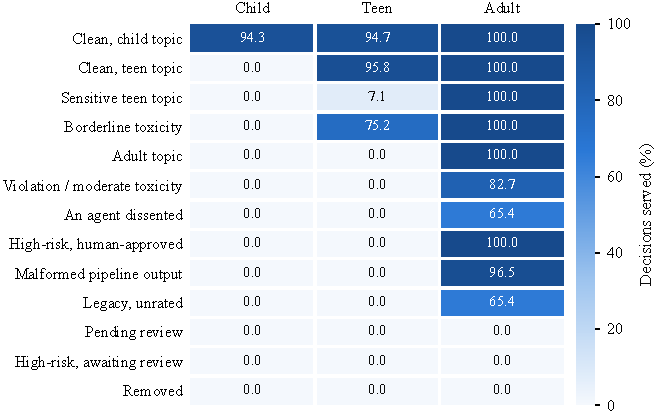
\includegraphics[width=\columnwidth]{fig_sweep}
\caption{Share of gate decisions that served the item, by item scenario and viewer tier, over all 64,000 profile--item pairs. No served item was a leak.}
\label{fig:sweep}
\end{figure}

Fig.~\ref{fig:reasons} shows why items were rejected. A rating above the viewer's tier accounts for 13,776 rejections (44.5\pct{}), blocked items for 5,120 and parental controls for 4,922. Only the first failing check is counted, so later checks look rarer than their reach.

\begin{figure}[t]
\centering
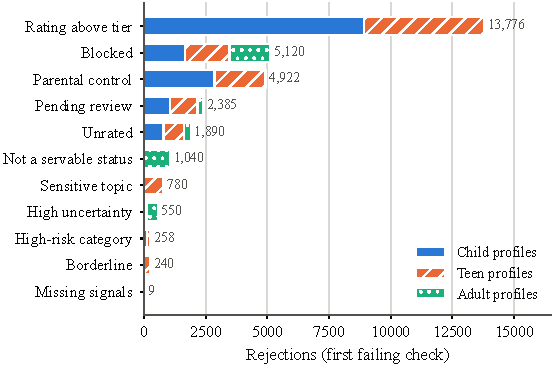
\includegraphics[width=\columnwidth]{fig_rejection_reasons}
\caption{The 30,970 rejections in the sweep by first failing check and viewer tier.}
\label{fig:reasons}
\end{figure}

Four randomised tests attacked the gate's stated properties, and none found a violation. (a) On 12,000 random profile--item pairs judged against an independent oracle, 1,540 items passed, 434 of them to minors, with no disagreement. (b) On 1,500 pairs, the gate decision was unchanged when interests, learned weights and history were removed. (c) On 1,040 feeds built through the full path with random interests, hostile learned weights, saturated history and a randomly trained bandit, 23,150 items were served, 15,495 to minors, with no leak. (d) A ranker constructed to inject rejected items, and one that rewrote ratings, had their additions removed by the final gate.

\subsection{What the Gate Prevents, and What It Cannot}

We generated five feeds of ten items for each child and teen profile, with the gate on and with the ranker applied to all items (Fig.~\ref{fig:leak}). Without the gate, 126 of 130 child feeds (96.9\pct{}) and 93 of 140 teen feeds (66.4\pct{}) contained a forbidden item. In item terms, 424 of 1,300 items served to children (32.6\pct{}) and 229 of 1,400 served to teens (16.4\pct{}) were forbidden. With the gate, none was.

\begin{figure}[t]
\centering
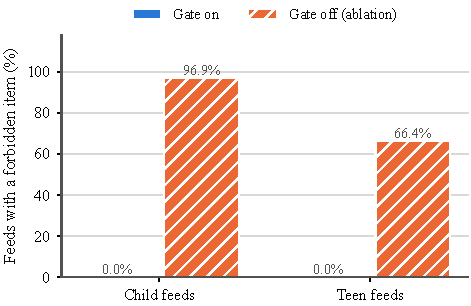
\includegraphics[width=\columnwidth]{fig_leak_rate}
\caption{Feeds containing at least one item the viewer must not see, with the gate and with the gate removed (130 child feeds, 140 teen feeds).}
\label{fig:leak}
\end{figure}

The gate has a clear limit. We marked a seeded 3\pct{} of clean-looking items as ones a later review would flag. The gate cannot detect them, and 24 of 130 child feeds (18.5\pct{}) and 19 of 140 teen feeds (13.6\pct{}) contained one. The 3\pct{} figure is an assumption, not a measurement, but the point holds for any rate: the gate enforces ratings and cannot correct a rating that is wrong.

\subsection{Cost}

The deterministic layer is cheap. Timed in memory on the laptop described above, rating derivation took a median of about 25\,$\mu$s per item and one gate decision about 23\,$\mu$s (64,000 decisions in 1.48\,s, up to 48,000 decisions per second). A full feed request (gate, ranking over an 800-item pool, gate again) took a median of 19.0\,ms and 23.3\,ms at the 95th percentile over 400 requests. These timings vary with machine load; a run taken while the machine was busy was about three times slower. No database, network or language-model call is included.

\subsection{Ranking and Learning}

Fig.~\ref{fig:relevance} compares one feed per profile against each profile's stated interests. Personalization clearly beats random selection among gate survivors (Precision@10 of 0.935 against 0.348; NDCG@10 of 0.863 against 0.261). It does not beat a plain sort by stated interests, which reaches a precision of 1.000 and an NDCG of 0.870. The precision gap is the diversity guard at work: it reserves 2 of 10 adult slots for topics outside the interests, giving $(26 \times 0.8 + 54 \times 1.0)/80 = 0.935$. Turning the bandit off raises NDCG to 0.892. We report this as a negative result.

\begin{figure}[t]
\centering
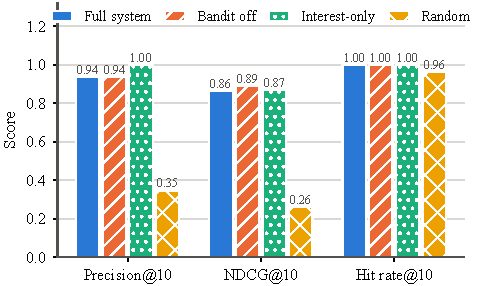
\includegraphics[width=\columnwidth]{fig_relevance}
\caption{Relevance of a single feed of 10 items against each profile's stated interests (80 profiles).}
\label{fig:relevance}
\end{figure}

To test learning, we simulated 36 viewers over 10 rounds of 10 items. Each clicks with probability 0.8 on two undeclared topics, 0.5 on declared interests and 0.05 otherwise, so only exploration can find the undeclared tastes (Fig.~\ref{fig:bandit}). For adults the full system reached a mean click rate of 0.454, against 0.435 with the bandit off and 0.408 with no learning, a relative gain of 11.2\pct{} over no learning. For teens the three variants were level (0.552, 0.553, 0.553) and for children also (0.554, 0.555, 0.548), which for children is consistent with the design, in which engagement cannot add topics. Random selection scored 0.343 for teens and 0.237 for adults. The simulation uses one seed, no confidence intervals were computed and the curves are visibly noisy, so differences of a few points should not be read as significant.

\begin{figure*}[t]
\centering
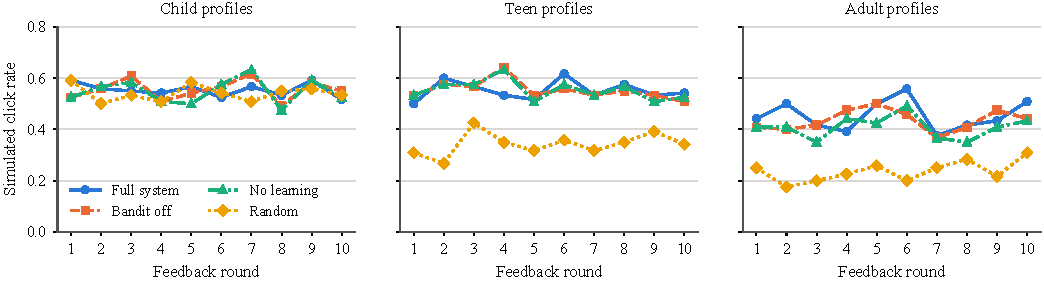
\includegraphics[width=\textwidth]{fig_bandit}
\caption{Simulated click rate per feedback round for 36 viewers with undeclared tastes. Learning helps adult profiles slightly and teen and child profiles not at all.}
\label{fig:bandit}
\end{figure*}

The guards held their limits (Fig.~\ref{fig:guards}). The borderline share was 5.7\pct{} for teen feeds against a 15\pct{} cap and 10.4\pct{} for adult feeds against a 30\pct{} cap, and it was zero for children under every system. Adult feeds had exactly the 20\pct{} minimum share outside stated interests, and covered 5.04 distinct topics per feed. The full system does not minimise borderline exposure: the interest-only sort served less (1.4\pct{} for teens and 3.5\pct{} for adults).

\begin{figure}[t]
\centering
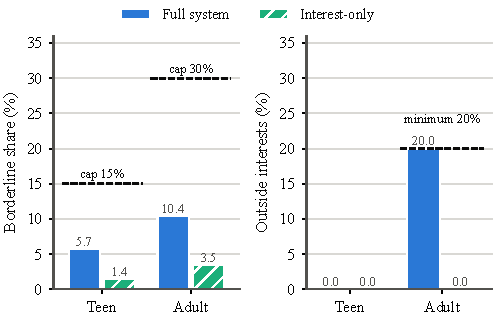
\includegraphics[width=\columnwidth]{fig_guards}
\caption{Drift and diversity guards. Left: share of each feed that is borderline-risk, with the tier caps. Right: share outside the viewer's stated interests, with the adult minimum.}
\label{fig:guards}
\end{figure}

\subsection{Moderator Queue and Precedents}

We ordered 64 queued items under three policies, reviewing one item per step, so time to review is queue position (Fig.~\ref{fig:queue}). High harm means a high-risk category awaiting review or toxicity of at least 0.5, which covers 35 items. The prioritizer reviewed high-harm items at a mean position of 20.0, against 22.6 for a risk-score sort and 42.6 for first-in-first-out, a 53.1\pct{} reduction against the latter. High-risk items were reached at a mean position of 12.5 against 52.5. Of the first 35 items reviewed, 88.6\pct{} were high-harm, against 74.3\pct{} and 28.6\pct{}. Exposure-weighted wait fell by 35.9\pct{} against first-in-first-out (1,466.9 against 2,289.2) and by 12.7\pct{} against the risk-score sort (1,680.8). Part of this follows from definitions: high-risk items are ordered first by rule and are included in the high-harm set.

\begin{figure}[t]
\centering
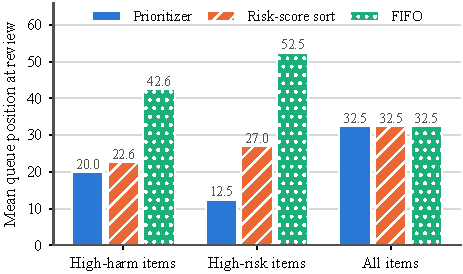
\includegraphics[width=\columnwidth]{fig_queue}
\caption{Mean queue position at which items are reviewed under three ordering policies (64 queued items; lower is sooner).}
\label{fig:queue}
\end{figure}

In a leave-one-out test over the 200 resolved cases with $k = 5$, the action suggested from precedents matched the moderator's in 66.0\pct{} of cases, against 40.0\pct{} for the rules alone (Fig.~\ref{fig:precedents}). This result is circular and should be read narrowly. The generator gives each category a house norm that the simulated moderator follows 80\pct{} of the time, and category-based retrieval recovers it. Rules alone score 0\pct{} on the 120 override cases by definition. The test shows that the mechanism works when such structure exists, and nothing more.

\begin{figure}[t]
\centering
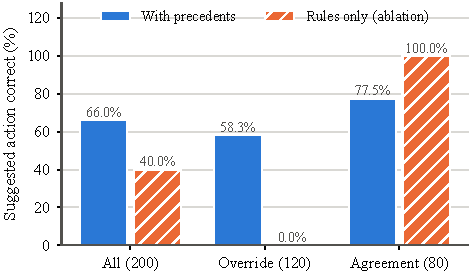
\includegraphics[width=\columnwidth]{fig_precedents}
\caption{Share of resolved cases in which the suggested action matched the moderator's final action, with and without precedent retrieval.}
\label{fig:precedents}
\end{figure}

\subsection{Adversarial Review}

Three review passes were run by independent reviewers who were given only the safety rules and the source code (Table~\ref{tab:review}). Together they found 12 leaks and 16 weaknesses.

\begin{table}[t]
\caption{Adversarial review passes. Weak.\ is weaknesses found.}
\label{tab:review}
\centering
\footnotesize
\begin{tabular}{@{}cp{0.27\columnwidth}ccp{0.3\columnwidth}@{}}
\toprule
Pass & Scope & Leaks & Weak. & Outcome \\
\midrule
1 & Rating and gate & 5 & 4 & all fixed \\
2 & Same, after fixes & 3 & 4 & all fixed \\
3 & Whole feature, new reviewer & 4 & 8 & all fixed except lost updates under concurrency \\
\bottomrule
\end{tabular}
\end{table}

The first two passes found leaks in rating derivation and label matching: missing signals were read as ``nothing found'', policy flags were ignored unless spelled exactly, spelling variants of high-risk labels slipped through, and a ``low'' parental strictness setting was looser than having no controls. In the third pass, the reviewer's 40,000-item fuzz of the gate itself found no violation. Every leak was in the code around it: one unreadable profile field dropped all parental controls, a failed mirror write left a stale copy that overrode a removal, a pipeline re-run undid a moderator's removal, and resolved high-risk cases were shown to ordinary moderators as precedents. Each finding now has a regression test. The fixes from the last pass were not independently re-checked.

\subsection{Live Run Through the Agentic Pipeline}

We sent 16 invented posts through the real workflow with the toxicity classifier on and a rule-based stand-in for the language model (Table~\ref{tab:live}). Nine were approved, four were held for human review, two were flagged and one was removed. The verified child profile was served 4 items, each teen 6 and each adult 9. Nothing flagged, held or removed was served to anyone.

\begin{table}[t]
\caption{Live run: 16 posts through the real pipeline. Tox.\ is the classifier's toxicity score.}
\label{tab:live}
\centering
\footnotesize
\begin{tabular}{@{}rp{0.34\columnwidth}cll@{}}
\toprule
\# & Post & Tox. & Status & Rating \\
\midrule
1 & Science fair volcano & 0.00 & approved & all ages \\
2 & Puppy at the zoo & 0.00 & approved & all ages \\
3 & Football match & 0.00 & approved & all ages \\
4 & Python bug fixed & 0.00 & approved & teen \\
5 & Phone review & 0.00 & approved & teen \\
6 & Exam stress & 0.00 & held & adult \\
7 & Election stock tips & 0.00 & held & adult \\
8 & Nightclub opening & 0.00 & approved & adult \\
9 & Personal insult & 0.99 & flagged & blocked \\
10 & ``Buy now'' offer & 0.00 & held & adult \\
11 & ``Secret truth'' cure & 0.00 & held & adult \\
12 & Insult to a referee & 0.87 & flagged & blocked \\
13 & Drawing with image & 0.00 & approved & adult \\
14 & Photos with image & 0.00 & approved & adult \\
15 & Suicide-prevention talk & 0.00 & removed & blocked \\
16 & Volcano puzzle & 0.00 & approved & all ages \\
\bottomrule
\end{tabular}
\end{table}

The run illustrates why a single classifier is not enough. The toxicity model scored 14 of the 16 posts at 0.00 and raised only the two insults. Of those 14, the other agents and rules held four for review (a sensitive topic twice, spam, and misinformation), removed one, and restricted three more to adults on topic or attached media. This is an illustration on 16 invented posts with a stand-in for the language model, not a comparison of accuracy, and one of the eight interventions is a false positive: the removed post announces a suicide-prevention talk and was caught by a keyword rule.

The run also found two defects that every synthetic test had passed. Approved content carries no enforcement action, because the enforcement agent is not run for it, and the rating required that field, so every clean post was rated adult. The synthesis step reports a weighted score of about 0.1 as its confidence, and the rating took the minimum confidence, so every item failed the uncertainty margin in (\ref{eq:margin}). On the first live run, before these fixes, feeds for minors were empty.

\section{Discussion}

\textbf{The safety value came from the deterministic layer.} A feed built from the gate and an interest sort would have scored as well on relevance and leaked as little. In an agentic system whose components are probabilistic and whose outputs are loosely typed, a small rule layer that can be enumerated and fuzzed is where assurance can be placed.

\textbf{Agents widen coverage and add failure modes.} The agentic pipeline covers harms a toxicity classifier does not score, and explains each verdict. It also produces free-form categories, omitted fields and confidences that mean different things in different agents. Both live-run defects were of this kind. Fail-closed derivation turns such faults into over-blocking, which is visible, in place of leaks, which are not.

\textbf{Review found more than testing did.} The tests and the code share an author and so share assumptions. Reviewers who had only the rules found twelve leaks the tests had missed, and the later ones were in storage and integration code that no gate test exercises.

\textbf{Synthetic data encodes its author's assumptions.} The live run broke two of them within 16 posts, in line with the finding of Kotarcic \emph{et al.} \cite{kotarcic2022human} that evaluation before deployment is not enough.

\section{Limitations and Ethics}
\label{sec:limits}

\textbf{Validity.} All evaluation data is synthetic and small in scale. A leak is defined on generator labels, so the gate is shown to respect ratings and signals, not to recognise harmful content. Relevance is defined from the same topic labels the rankers use. The language model is absent from every measured result; a real model emits free-form categories, most of which would be on no allow-list and rate adult, so feeds for minors would be sparse without a controlled topic vocabulary. This was not measured. We did not compare the agentic pipeline's classification accuracy with a supervised baseline. Most agents report a near-constant confidence, so the uncertainty margin is driven by disagreement between verdicts. The rating rules are tied to one pipeline's output fields.

\textbf{System.} Age is self-declared and not verified, and an account with no declared age group is treated as an adult. The gate trusts the moderation signals. Fail-closed design over-blocks: any image URL raises media risk in the host's heuristic and rates the post adult. Label matching is lexical and misses new slang, look-alike characters, other languages and text in images. Concurrent updates to profiles and bandit state can be lost. A moderator's approval plus hand-set tags can rate an item for children with no second check. Parental controls are set by an administrator, because the platform has no parent accounts.

\textbf{Ethics.} No real personal data was used and no human-subject data was collected. No harmful content was generated: harmful categories are represented by labels on placeholder text. Moderation targets conduct, such as violence, harassment, grooming and promotion of self-harm, and not political or religious belief. A gate like this can give false assurance. It does not replace age assurance or human moderation, and it should not be described as making a feed safe for children.

\section{Conclusion}

We described a platform that moderates content with cooperating agents in place of a single supervised classifier, and added an age-aware recommender to it by keeping the age decision outside every learned component. An audience rating that only rises, and a deterministic gate applied before and after ranking, withheld every above-tier item in 64,000 decisions and 1,040 feeds on synthetic data, at about 23\,$\mu$s per decision, while passing about 95\pct{} of the clean items minors were allowed to see. Removing the gate put a forbidden item in 96.9\pct{} of child feeds. The learned ranking contributed little beyond an interest sort. The most useful evidence came from outside the test suite: adversarial review found leaks in the code around the gate, and a single live run found two defects the synthetic data could not reveal.

Future work is, first, evaluation with a real language model and real content under ethical review, including a measured comparison of the agentic pipeline with a classifier baseline; then a controlled topic vocabulary, real engagement data with repeated seeds and confidence intervals, versioned storage, age assurance in place of self-declared age, a user study with moderators, and fairness across user and item groups.

\bibliographystyle{IEEEtran}
\bibliography{references}

\end{document}
